\documentclass[12pt]{article}
\usepackage[margin=1in]{geometry}
\geometry{letterpaper}                  
\usepackage{graphicx}
\usepackage[hyphens]{url}
\usepackage{fancyhdr}
%\pagestyle{fancy}
\usepackage{fixltx2e}
\usepackage{amsmath,amsfonts,amsthm,amssymb}
\usepackage{graphicx}
\usepackage{algorithm}
\usepackage{algorithmic}
\usepackage{url}
\usepackage[normalem]{ulem}
%\usepackage[pdftex]{color}
\usepackage{varioref}
\usepackage{mathrsfs}
\usepackage{amsmath}
\labelformat{equation}{\textup{(#1)}}
\usepackage[sort&compress,colon,square,numbers]{natbib}
%\usepackage{cite}


\usepackage{color}
\newcommand{\todo}[1]{{\color{red}{\it TODO: #1}}}

\DeclareMathOperator*{\argmin}{arg\,min}


\begin{document}

\begin{center}\Large \bf EN.580.694: Statistical Connectomics \\ Final Project Report \end{center}
\begin{center} Michael Norris $\cdot$  \today \end{center}
\bigskip


\subsection*{Using a Random Dot Product Model to Approximate the C. Elegans Connectome}
$\\ \\$
\centerline{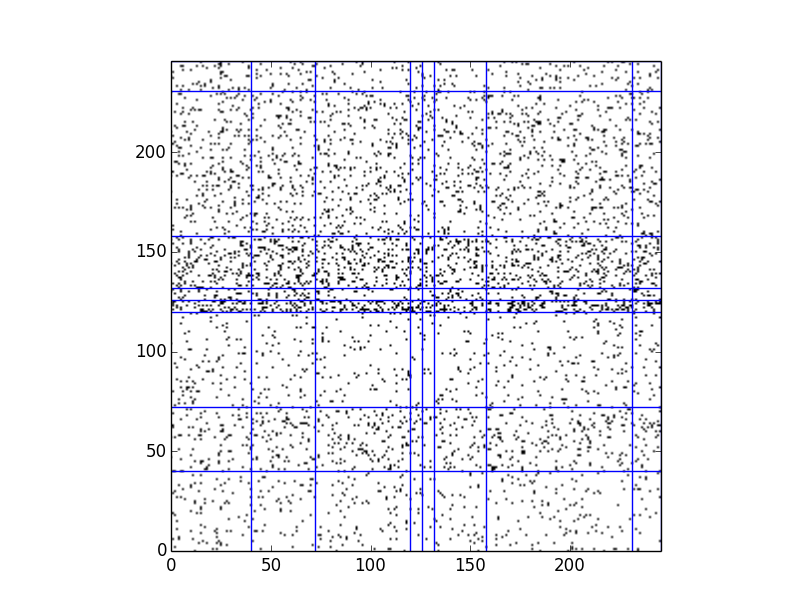
\includegraphics[scale=0.5]{adjacencymatrix.png}}
\newpage

\paragraph{Opportunity}
Graph Models allow us to generate similar graphs from a smaller amount of
parameters.  If we can model connectomes well, then a good model allows us to
generate similar connectomes to perform statistical analysis on similar graphs.
The paper by Pavlovic \cite{pavlovic} used the Erdos Reyni mixture model as an
approximation of the C. Elegans connectome.  Using other graph models to perform
the same analysis will aid future researchers in selecting tools for
connectomics work.

\paragraph{Challenge}

\paragraph{Action}
The Random Dot Product Graph Model (RDPG) represents each node by a random
vector, and assigns the probability of edges between nodes to be the dot product
between the two vectors \cite{young}.  

Here, we use a variant of RDPG, the Random Dot
Product Mixture Model, where we assign 

We use the block classifications from Figure 2 of \cite{pavlovic}, and generate
Random Dot Product Graphs with these blocks.

\paragraph{Resolution}
Shown above is the adjacency matrix that's the result of the parameter
estimation.  It's pretty bad for a few reasons.  First, the way that I organized
the RDP mixture model assigns a random vector to each vertex.  However, when we
block nodes, even if the blocks have their own $\alpha$ parameter, the dot
product between nodes in different blocks will probably be non-zero, and will
generate an edge with a somewhat higher than non-zero probability.



\paragraph{Future Work}
It would be cool to implement the same Random Dot Product Model with blocks that
have orthogonal or near-orthogonal vectors.  This would enable there to be fewer
edges between nodes in different blocks.  But this would require the ability to
generate orthogonal random vectors, or random near-orthogonal vectors with a
bounded probability by another parameter.

I also wrote code to do spectral embedding but did not get to play around with
that for clustering purposes.  It would be interesting to see how to do spectral
embedding for the different blocks in this model.

\newpage

\bibliography{main.bib}
\bibliographystyle{plain}


\end{document}  
